%%%%% Set up %%%%%

% Set document style and font size
\documentclass[12pt]{article}\usepackage[]{graphicx}\usepackage[]{color}
%% maxwidth is the original width if it is less than linewidth
%% otherwise use linewidth (to make sure the graphics do not exceed the margin)
\makeatletter
\def\maxwidth{ %
  \ifdim\Gin@nat@width>\linewidth
    \linewidth
  \else
    \Gin@nat@width
  \fi
}
\makeatother

\definecolor{fgcolor}{rgb}{0.345, 0.345, 0.345}
\newcommand{\hlnum}[1]{\textcolor[rgb]{0.686,0.059,0.569}{#1}}%
\newcommand{\hlstr}[1]{\textcolor[rgb]{0.192,0.494,0.8}{#1}}%
\newcommand{\hlcom}[1]{\textcolor[rgb]{0.678,0.584,0.686}{\textit{#1}}}%
\newcommand{\hlopt}[1]{\textcolor[rgb]{0,0,0}{#1}}%
\newcommand{\hlstd}[1]{\textcolor[rgb]{0.345,0.345,0.345}{#1}}%
\newcommand{\hlkwa}[1]{\textcolor[rgb]{0.161,0.373,0.58}{\textbf{#1}}}%
\newcommand{\hlkwb}[1]{\textcolor[rgb]{0.69,0.353,0.396}{#1}}%
\newcommand{\hlkwc}[1]{\textcolor[rgb]{0.333,0.667,0.333}{#1}}%
\newcommand{\hlkwd}[1]{\textcolor[rgb]{0.737,0.353,0.396}{\textbf{#1}}}%
\let\hlipl\hlkwb

\usepackage{framed}
\makeatletter
\newenvironment{kframe}{%
 \def\at@end@of@kframe{}%
 \ifinner\ifhmode%
  \def\at@end@of@kframe{\end{minipage}}%
  \begin{minipage}{\columnwidth}%
 \fi\fi%
 \def\FrameCommand##1{\hskip\@totalleftmargin \hskip-\fboxsep
 \colorbox{shadecolor}{##1}\hskip-\fboxsep
     % There is no \\@totalrightmargin, so:
     \hskip-\linewidth \hskip-\@totalleftmargin \hskip\columnwidth}%
 \MakeFramed {\advance\hsize-\width
   \@totalleftmargin\z@ \linewidth\hsize
   \@setminipage}}%
 {\par\unskip\endMakeFramed%
 \at@end@of@kframe}
\makeatother

\definecolor{shadecolor}{rgb}{.97, .97, .97}
\definecolor{messagecolor}{rgb}{0, 0, 0}
\definecolor{warningcolor}{rgb}{1, 0, 1}
\definecolor{errorcolor}{rgb}{1, 0, 0}
\newenvironment{knitrout}{}{} % an empty environment to be redefined in TeX

\usepackage{alltt}

% File path to resources (style file etc)
\newcommand{\locRepo}{csas-style}

% Style file for DFO Technical Reports
\usepackage{\locRepo/tech-report}

% header-includes from R markdown entry
\usepackage{float}

%%%%% Variables %%%%%

% New definitions: Title, year, report number, authors
% Protect lower case words (i.e., species names) in \Addlcwords{}, in "TechReport.sty"
\newcommand{\trTitle}{Quantifying shoreline modifications adjacent to eelgrass meadows in the Strait of Georgia Bioregion}
\newcommand{\trYear}{2022}
\newcommand{\trReportNum}{nnn}
% Optional
\newcommand{\trAuthFootA}{Email: \link{mailto:John.Cristiani@dfo-mpo.gc.ca}{\nolinkurl{John.Cristiani@dfo-mpo.gc.ca}} \textbar{} telephone: (250) 756-5555}
\newcommand{\trAuthsLong}{John M. Cristiani\textsuperscript{1} Katherine H. Bannar-Martin\textsuperscript{2} and Emily M. Rubidge\textsuperscript{2}}
\newcommand{\trAuthsBack}{Cristiani, J.C., Bannar-Martin, K.H, and Rubidge, E.M.}

% New definition: Address
\newcommand{\trAddy}{\textsuperscript{1}Pacific Biological Station\\
Fisheries and Oceans Canada, 3190 Hammond Bay Road\\
Nanaimo, British Columbia, V9T 6N7, Canada\\
\textsuperscript{2}Institute of Ocean Sciences\\
Fisheries and Oceans Canada, 9860 W Saanich Road\\
Sidney, British Columbia, V8L 4B2, Canada\\}

% Abstract
\newcommand{\trAbstract}{Here is the abstract text. Lorem ipsum dolor sit amet, consectetur adipisicing elit, sed do eiusmod tempor incididunt ut labore et dolore magna aliqua. Ut enim ad minim veniam, quis nostrud exercitation ullamco laboris nisi ut aliquip ex ea commodo consequat. Duis aute irure dolor in reprehenderit in voluptate velit esse cillum dolore eu fugiat nulla pariatur. Excepteur sint occaecat cupidatat non proident, sunt in culpa qui officia deserunt mollit anim id est laborum.}

% Resume (i.e., French abstract)
\newcommand{\trResume}{Voici le résumé. Lorem ipsum dolor sit amet, consectetur adipisicing elit, sed do eiusmod tempor incididunt ut labore et dolore magna aliqua. Ut enim ad minim veniam, quis nostrud exercitation ullamco laboris nisi ut aliquip ex ea commodo consequat. Duis aute irure dolor in reprehenderit in voluptate velit esse cillum dolore eu fugiat nulla pariatur. Excepteur sint occaecat cupidatat non proident, sunt in culpa qui officia deserunt mollit anim id est laborum.}

\newcommand{\trISBN}{}

\DeclareGraphicsExtensions{.png,.pdf}
%%%%% Start %%%%%

% Start the document
\IfFileExists{upquote.sty}{\usepackage{upquote}}{}

% commands and environments needed by pandoc snippets
% extracted from the output of `pandoc -s`
%% Make R markdown code chunks work
\usepackage{array}
\usepackage{amssymb,amsmath}
\usepackage{color}
\usepackage{fancyvrb}

% From default template:
\newcommand{\VerbBar}{|}
\newcommand{\VERB}{\Verb[commandchars=\\\{\}]}
\DefineVerbatimEnvironment{Highlighting}{Verbatim}{commandchars=\\\{\},formatcom=\color[rgb]{0.00,0.00,0.00}}
\usepackage{framed}
\definecolor{shadecolor}{RGB}{248,248,248}
\newenvironment{Shaded}{\begin{snugshade}}{\end{snugshade}}
\newcommand{\AlertTok}[1]{\textcolor[rgb]{0.94,0.16,0.16}{#1}}
\newcommand{\AnnotationTok}[1]{\textcolor[rgb]{0.56,0.35,0.01}{\textbf{\textit{#1}}}}
\newcommand{\AttributeTok}[1]{\textcolor[rgb]{0.77,0.63,0.00}{#1}}
\newcommand{\BaseNTok}[1]{\textcolor[rgb]{0.00,0.00,0.81}{#1}}
\newcommand{\BuiltInTok}[1]{#1}
\newcommand{\CharTok}[1]{\textcolor[rgb]{0.31,0.60,0.02}{#1}}
\newcommand{\CommentTok}[1]{\textcolor[rgb]{0.56,0.35,0.01}{\textbf{#1}}}
\newcommand{\CommentVarTok}[1]{\textcolor[rgb]{0.56,0.35,0.01}{\textbf{\textit{#1}}}}
\newcommand{\ConstantTok}[1]{\textcolor[rgb]{0.00,0.00,0.00}{#1}}
\newcommand{\ControlFlowTok}[1]{\textcolor[rgb]{0.13,0.29,0.53}{\textit{#1}}}
\newcommand{\DataTypeTok}[1]{\textcolor[rgb]{0.13,0.29,0.53}{#1}}
\newcommand{\DecValTok}[1]{\textcolor[rgb]{0.00,0.00,0.81}{#1}}
\newcommand{\DocumentationTok}[1]{\textcolor[rgb]{0.56,0.35,0.01}{\textbf{\textit{#1}}}}
\newcommand{\ErrorTok}[1]{\textcolor[rgb]{0.64,0.00,0.00}{\textit{#1}}}
\newcommand{\ExtensionTok}[1]{#1}
\newcommand{\FloatTok}[1]{\textcolor[rgb]{0.00,0.00,0.81}{#1}}
\newcommand{\FunctionTok}[1]{\textcolor[rgb]{0.00,0.00,0.00}{#1}}
\newcommand{\ImportTok}[1]{#1}
\newcommand{\InformationTok}[1]{\textcolor[rgb]{0.56,0.35,0.01}{\textbf{\textit{#1}}}}
\newcommand{\KeywordTok}[1]{\textcolor[rgb]{0.13,0.29,0.53}{\textit{#1}}}
\newcommand{\NormalTok}[1]{#1}
\newcommand{\OperatorTok}[1]{\textcolor[rgb]{0.81,0.36,0.00}{\textit{#1}}}
\newcommand{\OtherTok}[1]{\textcolor[rgb]{0.56,0.35,0.01}{#1}}
\newcommand{\PreprocessorTok}[1]{\textcolor[rgb]{0.56,0.35,0.01}{\textbf{#1}}}
\newcommand{\RegionMarkerTok}[1]{#1}
\newcommand{\SpecialCharTok}[1]{\textcolor[rgb]{0.00,0.00,0.00}{#1}}
\newcommand{\SpecialStringTok}[1]{\textcolor[rgb]{0.31,0.60,0.02}{#1}}
\newcommand{\StringTok}[1]{\textcolor[rgb]{0.31,0.60,0.02}{#1}}
\newcommand{\VariableTok}[1]{\textcolor[rgb]{0.00,0.00,0.00}{#1}}
\newcommand{\VerbatimStringTok}[1]{\textcolor[rgb]{0.31,0.60,0.02}{#1}}
\newcommand{\WarningTok}[1]{\textcolor[rgb]{0.56,0.35,0.01}{\textbf{\textit{#1}}}}
\begin{document}

%%%% Front matter %%%%%

% Add the first few pages
\frontmatter

%%%%% Drafts %%%%%

%\linenumbers  % Line numbers
%\onehalfspacing  % Extra space between lines
\renewcommand{\headrulewidth}{0.5pt}  % Header line
\renewcommand{\footrulewidth}{0.5pt}  % footer line
%\pagestyle{fancy}\fancyhead[c]{Draft: Do not cite or circulate}  % Header text

\newcommand{\lt}{\ensuremath <}
\newcommand{\gt}{\ensuremath >}

%Defines cslreferences environment
%Required by pandoc 2.8
%Copied from https://github.com/rstudio/rmarkdown/issues/1649
\newlength{\cslhangindent}
\setlength{\cslhangindent}{1.5em}
\newenvironment{cslreferences}%
  {}%
  {\par}

%%%%% Main document %%%%%
\hypertarget{introduction}{%
\section{Introduction}\label{introduction}}

The health and functioning of coastal marine ecosystems are under threat from a variety of human activities (\protect\hyperlink{ref-Halpern2019}{Halpern et al. 2019}). Coastal activities such as agriculture, industrial and residential development, forestry, and shoreline hardening can create pressures on the marine environment. A modified shoreline may alter levels of sedimentation, nutrient runoff, pollution, and wave energy (\protect\hyperlink{ref-Todd2019}{Todd et al. 2019}). For coastal biogenic habitat in British Columbia such as seagrass, these pressures may impact seagrass productivity and survival, and thus impact the community of species that rely on seagrass (\protect\hyperlink{ref-Iacarella2018}{Iacarella et al. 2018}; \protect\hyperlink{ref-Nahirnick2019}{Nahirnick et al. 2019}; \protect\hyperlink{ref-Murphy2021a}{Murphy et al. 2021}). Therefore, knowing the presence of shoreline modifications adjacent to seagrass would allow us to predict ecological impacts and understand seagrass ecosystem dynamics in a broader seascape context.

Assessing human activities for an entire coastal region is generally done at broad spatial scales. For example, impact mapping and assessments for all of BC have been done with a 2 km+ spatial resolution (\protect\hyperlink{ref-ClarkeMurray2015}{Clarke Murray et al. 2015}), which exceeds the size of many seagrass meadows as well as the size of the shoreline region which may be locally impacting a meadow. In addition, many spatially distinct meadows may exist close together, where only a high resolution assessment of shoreline modifications could distinguish the potential impacts between them. Fine-scale assessments of impacts to seagrass exist for the BC coast, but these are typically done in detail for only a few meadows due to logistical constraints (\protect\hyperlink{ref-Iacarella2018}{Iacarella et al. 2018}; \protect\hyperlink{ref-Nagel2020}{Nagel et al. 2020}).

The objective of this study is to map and quantify the shoreline modifications adjacent to all known seagrass meadows in the Strait of Georgia Bioregion of British Columbia. Eelgrass (\emph{Zostera marina}, the dominant habitat-forming seagrass species) is a conservation priority in British Columbia (\protect\hyperlink{ref-DFO2019}{DFO 2019}), and eelgrass meadows have been designated as Ecologically and Biologically Significant Areas (EBSA) due to their productivity, sensitivity, and support for biological diversity (\protect\hyperlink{ref-Rubidge2020}{Rubidge et al. 2020}). Therefore, it is important to acquire information on human activities to predict impacts and categorize meadows by their degree of naturalness, as areas of high naturalness may be a priority for additional management and conservation efforts (\protect\hyperlink{ref-UNCBD2008}{UN CBD 2008}). While shoreline modifications do not represent all of the human activities potentially threatening seagrass, a high resolution dataset is currently needed and can complement other existing human impact data.

\hypertarget{methods}{%
\section{Methods}\label{methods}}

\hypertarget{seagrass-spatial-data}{%
\subsection{Seagrass spatial data}\label{seagrass-spatial-data}}

Eelgrass (\emph{Z. marina}) is the primary subtidal and intertidal meadow-forming seagrass in British Columbia. Meadows may also consist of the non-native seagrass, \emph{Zostera japonica}, in the intertidal zone. Seagrass occurs to depths of 10 meters and can form meadows many km\textsuperscript{2} in size (\protect\hyperlink{ref-Murphy2021a}{Murphy et al. 2021}). We used a spatial dataset of seagrass in the Salish Sea compiled in Cristiani et al. (\protect\hyperlink{ref-Cristiani2021}{2021}), which consists of surveyed and modeled data from a variety of government and non-governmental sources. The dataset includes xyz meadows in the Strait of Georgia Bioregion as well as meadows in the southern portions of the Northern Shelf Bioregion and Southern Shelf Bioregion.

\hypertarget{shoreline-area}{%
\subsection{Shoreline area}\label{shoreline-area}}

Remember, the methods should be the most detailed part.
\begin{itemize}

\item
  Justification (cite DFO reports, Iacarella, Nagel)
\item
  Adjusting seagrass meadows (or just generally say we created it at the nearest shoreline)
\item
  General geoprocessing steps
\end{itemize}
We measured shoreline modifcations within at 100m buffer onto land from a seagrass meadow.

\ldots requires generating consistent buffers from onto land. The perimeter of the meadows, however, do not always abut directly to the shoreline due to different mapping accuracies and errors, thus resulting in slightly different buffer extents on to land. Aside from a few exceptions, the majority of meadows are adjacent to coastline and therefore to create consistent buffers we adjusted the perimeter of meadows to match the coastline using digitization tools in ArcGIS.

\hypertarget{shoreline-modifications}{%
\subsection{Shoreline modifications}\label{shoreline-modifications}}
\begin{itemize}

\item
  Modifications we are looking for and why (Emily's 2020 paper has some additional citations for impacts that I don't have)
\item
  Also, will need to say why I'm not including docks - its categorized elsewhere because of different impacts.
\item
  digitizing - general rules
\item
  attributes
\end{itemize}
\hypertarget{postprocessing}{%
\subsection{Postprocessing}\label{postprocessing}}
\begin{itemize}

\item
  Roads
\item
  General geoprocessing steps
\item
  Calculate as percentage of buffer and associate as attribute
\end{itemize}
\begin{figure}[H]

{\centering \pdftooltip{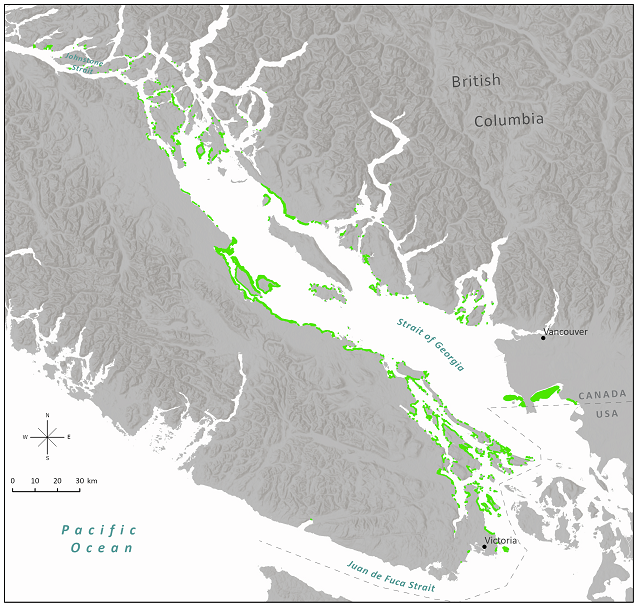
\includegraphics[width=6in]{figures/01_studyarea}}{Figure \ref{fig:studyareafig}} 

}

\caption{Study area}\label{fig:studyareafig}
\end{figure}
\hypertarget{results}{%
\section{Results}\label{results}}
\begin{itemize}

\item
  A few sentences on the spatial distribution (e.g.~more modifications in the south, more ag in south, more forestry in north).
\end{itemize}
\begin{figure}[H]

{\centering \pdftooltip{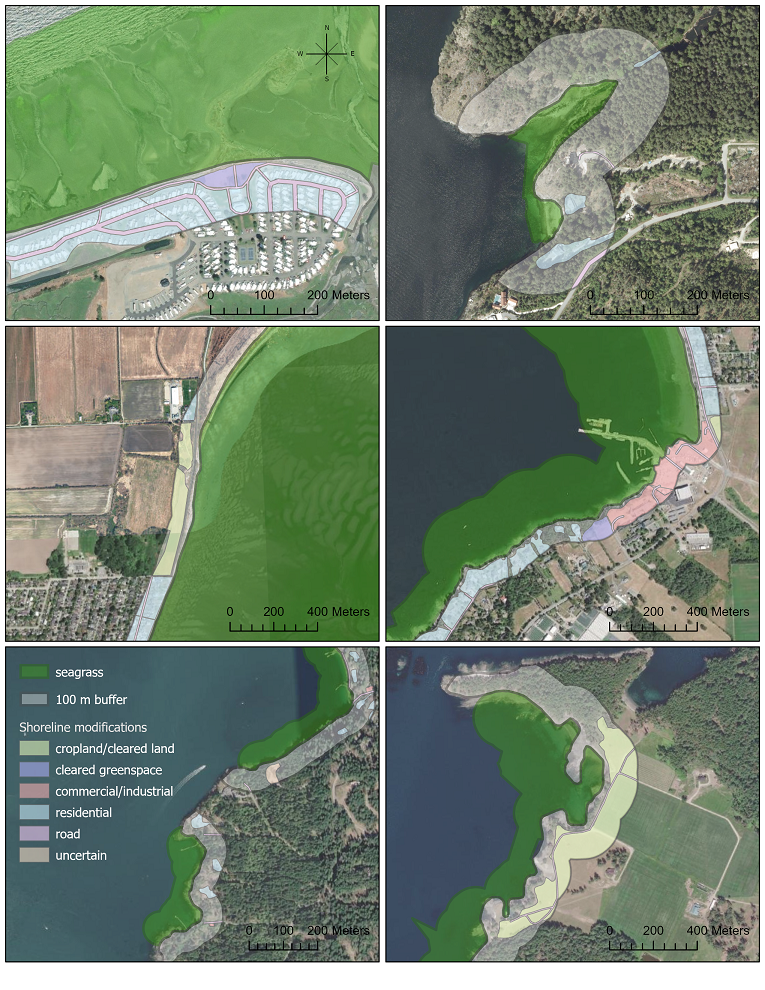
\includegraphics[width=6in]{figures/02_shorelinemod_examples}}{Figure \ref{fig:exampleareas}} 

}

\caption{Shoreline modifications within 100 meter buffered areas. The six selected areas are shown for example and do not imply any significance over other areas.}\label{fig:exampleareas}
\end{figure}
\begin{figure}[H]

{\centering \pdftooltip{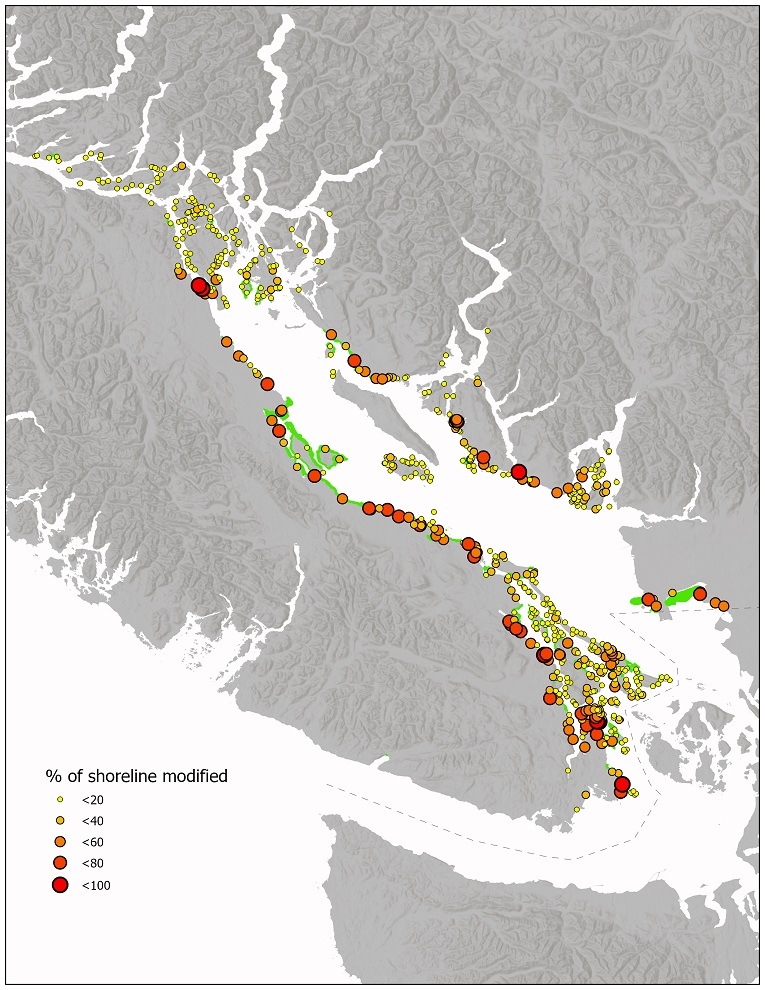
\includegraphics[width=6in]{figures/03_shorelinemod_percentage}}{Figure \ref{fig:percentmod}} 

}

\caption{The percentage of the shoreline buffer modified.}\label{fig:percentmod}
\end{figure}
\hypertarget{discussion}{%
\section{Discussion}\label{discussion}}
\begin{itemize}

\item
  summary paragraph
\item
  spatial distribution of activities and the significance for management
\item
  assumptions and limitations
  \begin{itemize}

  \item
    No point measurements in field to confirm impacts. Some activities are well regulated in Canada, like logging, and there may be very minimal impact.
  \item
    Meadows that aren't right on the coast may not experience any impacts
  \item
    If the modification exists behind some vegetation then the impact may be less (cite Iacarella)
  \item
    We use a uniform buffer, but there is a likely a distance decay for some of these activities.
  \end{itemize}
\item
  Future directions
  \begin{itemize}

  \item
    incorporate vulnerability scores to specific types of modifications
  \item
    Consider management goals of protecting the most natural meadows and how this might change given the spatial distribution of activities and other information (e.g.~biodiversity in meadows, connectivity)
  \end{itemize}
\item
  some stuff from my thesis:
  \begin{itemize}

  \item
    ``managing seagrass habitat and associated species in a landscape context, in which patterns of distribution, dispersal, and impacts will interact to influence regional management strategies (Murphy et al.~2021b). Although eelgrass is declining globally (Dunic et al.~2021), eelgrass in nearby Puget Sound, Washington is stable and resilient overall, despite a significant increase in local human and climactic stressors (Shelton et al.~2016). Assessing the relevance of managing for human impacts in the Salish Sea will therefore require a deeper understanding of seagrass and invertebrate responses to stressors and the mechanisms (e.g., dispersal) that allow for resilience to these stressors. Ultimately, refining and validating our models will increase their utility and promote their incorporation into broader marine spatial planning efforts.''
  \end{itemize}
\end{itemize}
\clearpage

\hypertarget{references}{%
\section{References}\label{references}}

\noindent \vspace{-2em} \setlength{\parindent}{-0.2in} \setlength{\leftskip}{0.2in} \setlength{\parskip}{8pt}

\hypertarget{refs}{}
\begin{CSLReferences}{1}{0}
\leavevmode{\hypertarget{ref-ClarkeMurray2015}{}}%
Clarke Murray, C., Agbayani, S., Alidina, H.M., and Ban, N.C. 2015. \link{https://doi.org/10.1016/j.marpol.2015.04.003}{Advancing marine cumulative effects mapping: {An} update in {Canada}'s {Pacific} waters}. Marine Policy 58: 71--77.

\leavevmode{\hypertarget{ref-Cristiani2021}{}}%
Cristiani, J., Rubidge, E., Forbes, C., Moore-Maley, B., and O'Connor, M.I. 2021. \link{https://doi.org/10.3389/fmars.2021.717469}{A {Biophysical Model} and {Network Analysis} of {Invertebrate Community Dispersal Reveals Regional Patterns} of {Seagrass Habitat Connectivity}}. Frontiers in Marine Science 8: 1--19.

\leavevmode{\hypertarget{ref-DFO2019}{}}%
DFO. 2019. Design strategies for the {Northern Shelf Bioregion Marine Protected Area Network}. CSAS.

\leavevmode{\hypertarget{ref-Halpern2019}{}}%
Halpern, B.S., Frazier, M., Afflerbach, J., Lowndes, J.S., Micheli, F., O'NAHara, C., Scarborough, C., and Selko, K.A. 2019. \link{https://doi.org/10.1038/s41598-019-47201-9}{Recent pace of change in human impact on the world's ocean}. Scientific Reports 9(1): 1--8.

\leavevmode{\hypertarget{ref-Iacarella2018}{}}%
Iacarella, J.C., Adamczyk, E., Bowen, D., Chalifour, L., Eger, A., Heath, W., Helms, S., Hessing-Lewis, M., Hunt, B.P.V., MacInnis, A., O'Connor, M.I., Robinson, C.L.K., Yakimishyn, J., and Baum, J.K. 2018. \link{https://doi.org/10.1111/gcb.14090}{Anthropogenic disturbance homogenizes seagrass fish communities}. Global Change Biology 24(5): 1904--1918.

\leavevmode{\hypertarget{ref-Murphy2021a}{}}%
Murphy, G.E.P., Dunic, J.C., Adamczyk, E.M., Bittick, S.J., Côt'e, I.M., Cristiani, J., Geissinger, E.A., Gregory, R.S., Lotze, H.K., O'Connor, M.I., Ara'ujo, C.A.S., Rubidge, E.M., Templeman, N.D., and Wong, M.C. 2021. \link{https://doi.org/10.1139/facets-2020-0020}{From coast to coast to coast~: Ecology and management of seagrass ecosystems across {Canada}}. Facets 6: 1--41.

\leavevmode{\hypertarget{ref-Nagel2020}{}}%
Nagel, E.J., Murphy, G.E.P., Fast, J., Bittick, S.J., Adamczyk, M., Connor, M.I.O., Wong, M.C., and Lotze, H.K. 2020. Application of a coastal human impact metric and nitrogen loading model to 10 eelgrass ( {Zostera} marina ) meadows in {British Columbia}. {Fisheries and Oceans Canada}.

\leavevmode{\hypertarget{ref-Nahirnick2019}{}}%
Nahirnick, N.K., Costa, M., Schroeder, S., and Sharma, T. 2019. \link{https://doi.org/10.2112/jcoastres-d-18-00112.1}{Long-{Term Eelgrass Habitat Change} and {Associated Human Impacts} on the {West Coast} of {Canada}}. Journal of Coastal Research 36(1): 30.

\leavevmode{\hypertarget{ref-Rubidge2020}{}}%
Rubidge, E., Jeffery, S., Gregr, E.J., Gale, K.S.P., and Frid, A. 2020. Assessment of nearshore features in the {Northern Shelf Bioregion} against criteria for determining {Ecologically} and {Biologically Significant Areas} ( {EBSAs} ). DFO Canadian Science Advisory Secretariat. {Canadian Science Advisory Secretariat}.

\leavevmode{\hypertarget{ref-Todd2019}{}}%
Todd, P.A., Heery, E.C., Loke, L.H.L., Thurstan, R.H., Kotze, D.J., and Swan, C. 2019. \link{https://doi.org/10.1111/oik.05946}{Towards an urban marine ecology: Characterizing the drivers, patterns and processes of marine ecosystems in coastal cities}. Oikos: 1215--1242.

\leavevmode{\hypertarget{ref-UNCBD2008}{}}%
UN CBD. 2008. Decision adopted by the conference of the parties to the convention on biological diversity at its ninth meeting. UNEP/CBD/COP/DEC/IX/20.

\end{CSLReferences}
\end{document}
